\section{Síntesis e implementación}
El diseño se sintetizó e implementó con Vivado para la FPGA Artix-7 (XC7A35T) de la Basys 3.

\subsection{Utilización de recursos}
La Tabla~\ref{tab:utilizacion} resume los recursos utilizados luego de la implementación, y la Figura~\ref{fig:utilizacion} muestra el reporte jerárquico obtenido en Vivado, discriminado por módulo.

\begin{table}[H]
	\centering
	\caption{Utilización de recursos post-implementación.}
	\label{tab:utilizacion}
	\begin{tabular}{lrrrr}
		\toprule
		\textbf{Recurso} & \textbf{top (total)} & \textbf{u\_alu} & \textbf{Disponible} & \textbf{Utilización} \\
		\midrule
		Slice LUTs        & 77 & 74 & 20800 & 0,37\,\% \\
		Slice Registers   & 22 & 0  & 41600 & 0,05\,\% \\
		F7 Muxes          & 11 & 11 & 16300 & 0,07\,\% \\
		Slices            & 23 & 22 & 8150  & 0,28\,\% \\
		Bonded IOB        & 23 & 0  & 106   & 21,70\,\% \\
		BUFGCTRL          & 1  & 0  & 32    & 3,13\,\% \\
		\bottomrule
	\end{tabular}
\end{table}

\begin{figure}[H]
	\centering
	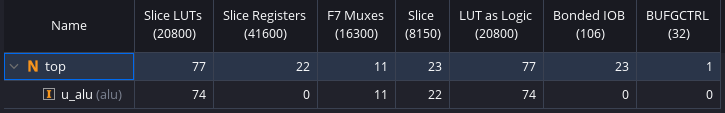
\includegraphics[width=0.9\textwidth]{img/utilizacion.png}
	\caption{Reporte de utilización jerárquico en Vivado.}
	\label{fig:utilizacion}
\end{figure}

Del reporte se desprenden algunas observaciones:
\begin{itemize}
	\item La cantidad de registros es exactamente 22, que coincide con los bits de A, B y opcode ($2 \cdot \texttt{MSB} + 6 = 22$ para 8 bits). Todos pertenecen al módulo top: la ALU no utiliza ningún registro, lo que confirma que se sintetizó como lógica puramente combinacional y que no se infirieron \textit{latches}.
	\item Prácticamente toda la lógica (74 de las 77 LUTs) corresponde a la ALU. Las 3 LUTs restantes pertenecen al módulo top y corresponden a la lógica de carga de los registros (decodificación de \texttt{i\_abc} y reset).
	\item Los 11 multiplexores F7 son utilizados por la ALU para combinar las salidas de LUTs, lo que es consistente con la selección del resultado entre las distintas operaciones y con los desplazadores, que son esencialmente redes de multiplexores.
	\item Los 23 IOB corresponden a los puertos del top: 8 de \texttt{i\_datos}, 3 de \texttt{i\_abc}, \texttt{i\_reset}, \texttt{clock}, 8 de \texttt{o\_led}, \texttt{o\_zero} y \texttt{o\_overflow}. El único BUFG es el buffer global del reloj.
\end{itemize}

En conjunto, el diseño ocupa una fracción ínfima de la FPGA, lo que deja amplio margen para integrarlo en el procesador del trabajo final.

\subsection{Análisis de tiempos}
\label{sec:tiempos}
La Figura~\ref{fig:timing} muestra el \textit{Timing Summary} obtenido luego de la implementación.

\begin{figure}[H]
	\centering
	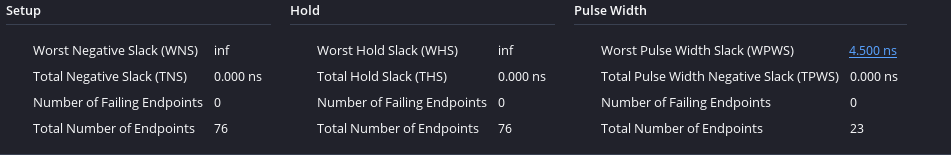
\includegraphics[width=\textwidth]{img/timing_summary.png}
	\caption{Resumen de tiempos post-implementación.}
	\label{fig:timing}
\end{figure}

Tanto el WNS como el WHS resultan infinitos y no hay ningún \textit{endpoint} que falle. Esto no significa que el diseño tenga un margen ilimitado, sino que \textbf{no existe ningún camino restringido por el reloj}:
\begin{itemize}
	\item Los caminos desde los \textit{switches} hasta los registros A, B y opcode parten de puertos de entrada sin \texttt{set\_input\_delay}.
	\item Como las salidas de la ALU no se registran, los caminos que la atraviesan parten de los registros y terminan directamente en los pines de los LEDs, que no tienen \texttt{set\_output\_delay}.
\end{itemize}
Al no haber caminos registro a registro, Vivado no tiene contra qué comparar los retardos, y los 76 \textit{endpoints} quedan sin restricción.

El único parámetro con un valor finito es el \textit{Worst Pulse Width Slack} (WPWS) de 4,5~ns, que verifica que los pulsos alto y bajo del reloj de 100~MHz (5~ns cada uno) sean más largos que el mínimo exigido por los \textit{flip-flops}. Con este margen, el reloj de la placa no representa ninguna limitación.

Si bien estos caminos no se comparan contra el período del reloj, Vivado igualmente calcula su retardo. Para obtenerlo se analizaron los caminos que van desde los registros A, B y opcode hasta las salidas.

El camino más largo, en la esquina de proceso lenta, va desde \texttt{A\_reg[2]} hasta \texttt{o\_zero}, con un retardo de datos de 15,149~ns (5,766~ns de lógica y 9,382~ns de ruteo) y 8 niveles lógicos. La Tabla~\ref{tab:camino_critico} muestra su desglose.

\begin{table}[H]
	\centering
	\caption{Desglose del camino crítico \texttt{A\_reg[2]} $\rightarrow$ \texttt{o\_zero}. Los tiempos son acumulados desde el flanco de reloj en el pin W5.}
	\label{tab:camino_critico}
	\begin{tabular}{llr}
		\toprule
		\textbf{Etapa} & \textbf{Recursos} & \textbf{Tiempo (ns)} \\
		\midrule
		Distribución del reloj hasta el registro & IBUF, BUFG & 5,154 \\
		Salida del registro A & FDRE & 5,610 \\
		Sumador/restador & LUT2, 2 $\times$ CARRY4 & 7,600 \\
		Selección del resultado según el opcode & LUT5, MUXF7, LUT6 & 10,188 \\
		Detección de cero & LUT6 & 11,294 \\
		Ruteo hasta el pin L1 & -- & 16,781 \\
		Buffer de salida & OBUF & 20,303 \\
		\bottomrule
	\end{tabular}
\end{table}

El camino es coherente con la estructura del diseño: atraviesa la suma (implementada con las cadenas de acarreo \texttt{CARRY4}), el multiplexor que elige el resultado según el opcode, y finalmente la compuerta que detecta si el resultado es cero, que necesita conocer todos los bits del resultado y por eso es la salida más lenta. Los caminos siguientes son los de \texttt{o\_overflow} (11,413~ns) y \texttt{o\_led[5]} (10,630~ns).

Se observa además que la lógica de la ALU propiamente dicha, desde la salida del registro hasta la detección de cero, demora unos 5,7~ns. El resto del retardo corresponde a la distribución del reloj, al ruteo hasta el pin (5,5~ns, ya que el LED LD15 está alejado de la lógica) y al buffer de salida (3,5~ns).

Si en el procesador del trabajo final se necesita garantizar que la ALU opere dentro de un ciclo de reloj, bastará con registrar su salida (o las entradas de la etapa siguiente). De esa forma el camino pasa a ser registro a registro y el análisis de tiempos arroja un WNS real. Con unos 5,7~ns de lógica, es esperable que la ALU entre holgadamente en el período de 10~ns, aunque esto deberá confirmarse con el análisis de tiempos del diseño final, ya que el ruteo dependerá de la ubicación de la lógica.
